%-----------------------------
% CSCI 315, Spring 2018
% 
% Aaron Pfister
% Language: Ruby
%-----------------------------
% * <apfister2@mail.csuchico.edu> 2018-03-24T19:31:08.831Z:
%
% ^.

\documentclass{article}
%-----------------------------
% List of Packages 
%-----------------------------
\usepackage{graphicx}   % Need for images
\usepackage{caption}     % Useful to suppress caption numbers with *
\usepackage{listings}      % Needed for code and syntax highlighting
\usepackage{multicol}     % Permits sections with multiple columns
\usepackage{enumitem}  % More options for itemize, enumerate, and description
\usepackage{hyperref}            % For nice urls
\usepackage{tikz}            % For drawing cool things

%-----------------------------
% Set Settings and Macros
%-----------------------------

% define some custom colors
\definecolor{comment_green}{rgb}{0,0.6,0}
\definecolor{numbers_gray}{rgb}{0.5,0.5,0.5}
\definecolor{string_mauve}{rgb}{0.58,0,0.82}

% This is the default columnsep (from multicolums)
\setlength\columnsep{30pt} 

% Configure code and syntax highlighting
% Not all languages supported (but many are)
% Find the language closest to yours, and extend it with morekeywords
% Recommended reference: https://en.wikibooks.org/wiki/LaTeX/Source_Code_Listings
\lstset{%
    language=Ruby,   
    basicstyle=\small,                                          % the size of the fonts that are used for the code
    commentstyle=\color{comment_green},       % comment style
    keywordstyle=\color{blue},                          % keyword style
    morekeywords={*,...},                                 % if you want to add more keywords to the set
    stringstyle=\color{string_mauve},                % string literal style
    numberstyle=\tiny\color{numbers_gray},        % the style that is used for the line-numbers
    numbers=left,                                            % where to put the line-numbers; possible values are (none, left, right)
    numbersep=6pt,
    frame=single, % adds a frame around the code
    keepspaces=true,
    tabsize=2	                                                     % sets default tabsize to 4 spaces
}

\begin{document}
%-----------------------------
% Header
%-----------------------------
\title{D\&D Dice Roller \\ \large{\sc CSCI 315, Programming Languages}}
\author{Aaron Pfister}
\date{Spring 2018}
\maketitle
% Use tikz to add some images outside the normal printing area
\begin{tikzpicture}[remember picture,overlay]
   % This sets logo in upper right corner (optional)
   \node[anchor=north east,inner sep=40pt] at (current page.north east)
             {
\includegraphics[scale=0.36]{ddo2}};
   \draw (-4,1) -- (15,1);
\end{tikzpicture}

%-----------------------------
% Ruby
%-----------------------------
\section*{Ruby}
This lab is designed to use the Ruby programming language. Directions for downloading and installing ruby: \href{https://www.ruby-lang.org/en/documentation/installation/}{\underline{https://www.ruby-lang.org/en/documentation/installation/}}

%-----------------------------
% Overview
%-----------------------------
\section*{Overview}
The goal of this lab is to create a 2 player (Human vs. Machine, Human vs. Human, Machine vs. Machine), turn based dice rolling game. The object of the game is to knock your opponent down more times than they knock you down. My inspiration for this lab comes from turn based video games and a dungeons and dragons video game I used to play. I also believe the turn based style is easier to think about, plan out and implement in code. Since Ruby is object-oriented, this lab will utilize classes and inheritance. 

%-----------------------------
% Attack Module
%-----------------------------
\section*{Attack Module}
First you will need to create the module for Attack, which will hold methods for using a weapon. Attack will hold 2 methods: \textbf{try\_hit} and \textbf{damage}. The \textbf{try\_hit} method will take an integer, hit\_chance, as its parameter and use the rand() function to pick a number between 1 and 100. The method will return true if the random number is greater than hit\_chance and false if it is less. The \textbf{damage} method will take two integers for its parameters, damage\_modifier and dice. The method uses the rand function to pick a number between 1 and dice and multiplies this number by the damage modifier, and returns the result.
\newpage

%-----------------------------
% Weapon Class
%-----------------------------
\section*{Weapon Class}
Next you will start creating the class for Weapon. The Weapon class has four instance variables: \textbf{name, hit\_chance, damage\_modifier, dice}. \textbf{hit\_chance} stores the lowest number a player can roll and still hit their opponent. \textbf{dice} is the size of the dice and \textbf{damage\_modifier} is the number multiplied by the dice to determine overall damage of a swing. The constructor will take a string and 3 integers to be set to the corresponding member variables. \\
\\
For the Weapon class, you will need to create the \textbf{swing} method that returns the total damage when \textbf{try\_hit} returns true, and 0 when it returns false. \\
You can use the method \textbf{attr\_accessor} in order to create getter and setter functions for member variables of your class. For example: \\
\begin{lstlisting}
class Class
	attr_accessor :m_var #single variable
    attr_accessor :m_var2, :m_var3 #multiple variables
    
    def initialize(m_var, m_var2, m_var3)
    	@m_var, @m_var2, @m_var3 = m_var, m_var2, m_var3
    end
end

c1 = Class.new(1, 2, 3)
puts "#{c1.m_var}" # => 1
c1.m_var = 2 
puts "#{c1.m_var}" # => 2
\end{lstlisting}

%-----------------------------
% Player Class
%-----------------------------
\section*{Player Class}
The Player class contains 2 subclasses: Human and Machine. \\
Player will have 3 instance variables: \textbf{health, weapons\_list, wins}. \textbf{weapons\_list} holds the 3 different weapons available to the player at the beginning of each round. Both\textbf{health} and \textbf{wins} will be updated and maintained throughout the game. The constructor will take an integer and an array of weapons to be set to \textbf{health} and \textbf{weapons\_list}, and \textbf{wins} will be set to 0. \\

\subsection*{Human Class}
Human contains 1 more instance variable: \textbf{name}. The constructor will take and integer on top of the Player class constructor. \\
The \textbf{set\_weapon} method will be necessary for this class. This method will prompt the user to choose a weapon and then set the Players weapon to that choice. 

\textbf{Tip: Using attr\_accessor :weapon will provide functions available to the Weapon class.}

\subsection*{Machine Class}
The Machine class constructor takes the same parameters as the Player class, but, upon instantiation, will set a random weapon from \textbf{weapons\_list} and \textbf{name} to Machine. \\
The \textbf{set\_weapon} method will choose a random weapon from \textbf{weapons\_list} and set it as the new weapon. 

%-----------------------------
% Game Layout
%-----------------------------
\section*{Game Layout}
\begin{enumerate}

\item Each game will start with a picture using the Catpix gem. Instructions and information about the gem can be found \href{https://github.com/pazdera/catpix}{\underline{here}}. It is as simple as: \\
\begin{lstlisting}
require 'catpix'

Catpix::print_image "dice.jpg", 
	:limit_x => 0.5,
	:limit_y => 0,
	:center_x => true,
	:center_y => true,
	:bg => "white",
	:bg_fill => false,
	:resolution => "high"
\end{lstlisting}
\textbf{Note: I was not able to find a better gem to use. Unfortunately the picture quality is not great, but increasing terminal window size will result in better quality.}

\item Ask the user to input 3 \textbf{weapon}s for the Machine \textbf{weapons\_list}, then 3 weapons for the Human weapons list. You can assume that there will always be three weapons and there will be no bad input.

\item Ask the user to enter the starting \textbf{health} and \textbf{name} for each Player. After this, Player objects can be declared. If the user enters "Machine", the type of Player will be Machine. Next, ask the user how many rounds they would like to play.

\item After the initial information is recorded, the game may begin. For each round: \\
\newpage
\begin{enumerate}
\item Set weapon of each player.
\item Print out picture signifying the start of a round.
\item Make each player swing their weapon.
\item Update/maintain \textbf{health} and \textbf{wins} of each player.
\item Repeat c and d until the \textbf{health} of one of the Players reaches 0.
\end{enumerate}

\item Once each round has been played, a summary of each round should be printed to the screen. For example: \\
\begin{lstlisting}
Lochenih won round 1 using a Longsword.
Lochenih won round 2 using a Mace.
Lochenih won round 3 using a Rapier.
\end{lstlisting}

\item Lastly, the winner should be announced, and the program will end.
\begin{center}
    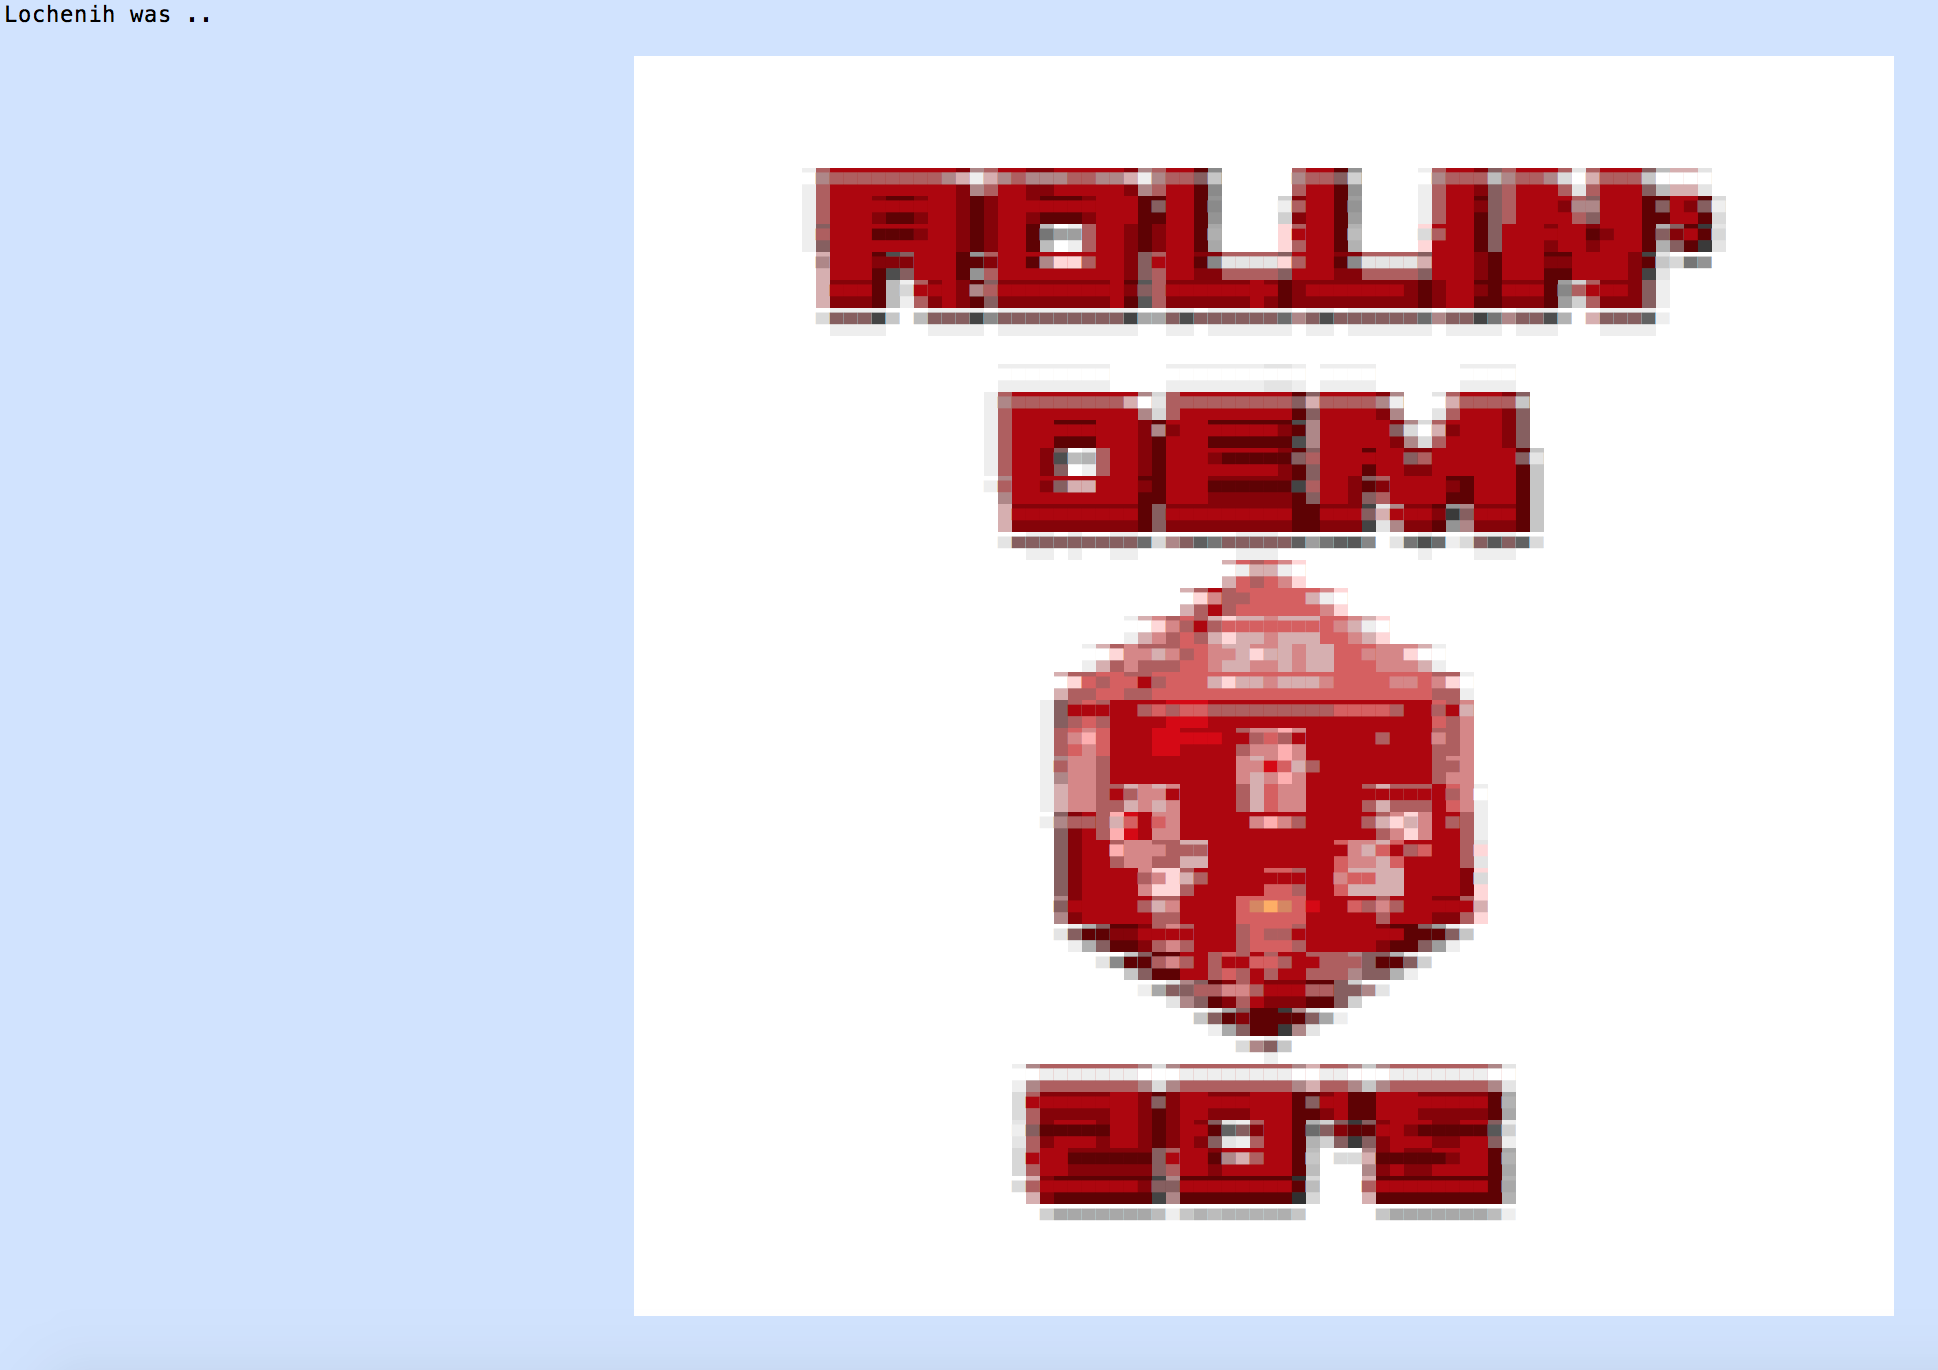
\includegraphics[width=0.8\textwidth]{end}
\end{center}

\end{enumerate}

%-----------------------------
% Testing and Troubleshooting
%-----------------------------
\section*{Testing and Troubleshooting}
Since the outcome of each test may change from time to time, you should make sure your program is printing the correct strings at the correct times. For each test, your output should match up to the beginning of each round. I recommend using the Internet to become familiar with Ruby before starting the lab. \\
You can use the piping method in order to run test inputs:
\begin{center}
\textbf{ruby game.rb $<$ tests/t01.in}
\end{center}

%-----------------------------
% Given
%-----------------------------
\section*{Files Provided}
Each student will be given a starter pack containing 2 files (starter\_weapon.rb and starter\_player.rb), a tests folder, and images to use in the program.

%-----------------------------
% Turning it in
%-----------------------------
\section*{Submission}
Each student will work on the project individually and submit your program (\textbf{weapon.rb player.rb game.rb}) via Blackboard or email. Programs will be graded manually based on use of classes, Catpix, and other features of the  Ruby language, along with commenting and cleanliness of code.

\end{document}

